\RequirePackage{plautopatch}  % pLaTeX または upLaTeX のとき
%\documentclass[uplatex,dvipdfmx,titlepage,a4j]{jsarticle}% upLaTeX のとき
\documentclass[dvipdfmx,titlepage,a4j]{jsarticle}  % pLaTeX のとき
\usepackage{listings,jvlisting}
\usepackage{amsmath,amssymb}
\usepackage{graphicx}
\usepackage[yen]{okuverb}
\usepackage{r04ec-exp}
\usepackage{here}
\usepackage{ascmac}
\usepackage{fancybox}
\usepackage{fancyvrb}
\usepackage{fancyhdr}
\usepackage{lastpage}
\usepackage{cases}
\usepackage[hang,small,bf]{caption}
\usepackage[subrefformat=parens]{subcaption}

\captionsetup{compatibility=false}

\fancypagestyle{foot}
{
\fancyhead[L]{}
\fancyhead[C]{数値シミュレーション}
\fancyhead[R]{}
% \fancyfoot[C]{\thepage / \pageref{LastPage}}
\renewcommand\headrulewidth{0.4pt}
}

%ここからソースコードの表示に関する設定
\lstset{
  language={C++},
  basicstyle={\ttfamily},
  identifierstyle={\small},
  commentstyle={\smallitshape},
  keywordstyle={\small\bfseries},
  ndkeywordstyle={\small},
  stringstyle={\small\ttfamily},
  frame={tb},
  tabsize={2},
  breaklines=true,
  columns=[l]{fullflexible},
  numbers=left,
  xrightmargin=0zw,
  xleftmargin=3zw,
  numberstyle={\scriptsize},
  stepnumber=1,
  numbersep=1zw,
  lineskip=-0.5ex
}

\renewcommand{\lstlistingname}{リスト}
%ここまでソースコードの表示に関する設定

\title{数値シュミレーション}
% 学年・番号
\grade{4年42番}%
% 氏名
\author{鷲尾 優作}
% 班(後期は班に分かれて実験をする.そのときは,ここに班番号を記入する.)
\team{}
% 提出日
\date{2022年10月3日}
% 実験日
\expdate{2022年10月20日}
% 共同実験者
% グループに分かれて実験をするテーマでは,グループメンバーの番号名前を書く.
\coauthor{}
%
%記載例:
%\coauthor{%
%  2番 & 新潟 花子\\
%  11番 & 三条 次郎}
%%

\begin{document}
\pagestyle{foot}

\maketitle

\section{目的}
これまでの実験・講義では解析的に系の挙動を明らかにすることができるモデルを扱ってきた.

しかしながら,二重振り子をはじめとした複雑な系では従来の解析方法が適用できない場合が存在し,
この場合,エネルギ式を用いての運動方程式の導出や数値モデルを利用した運動シミュレーションが有効とされている.
同技術には,系の挙動の解析のみならず,安定化や安全性の向上に用いる制御器の制御パラメータの導出がコンピュータ上で行える利点がある.

ここでは,電気系・力学系のシミュレーションモデルをScilab上で構成し,解析結果の有効性確認方法・対象の制御パラメータの調整法を確認する.

\section{バネ-マス-ダンパ系のシミュレーション}
本来数値シミュレーションを必要とするのはより複雑な系の解析であるが,ここでは単純なバネ-マス-ダンパ系のシミュレーションモデルを
構成し,モデルの構成方法・出力の評価が正しく実施できることを確認する.

天井の固定点からバネ$k$[kg/s$^2$]でダンパ$c$[kg/s]で支持された質量$m$[kg]から
なる系を考える.質量の運動は上下方向のみとし,重力と空気抵抗の影響は受けないものとする.
この系に対し,ステップ状の外力$f(t) = f_o \cdot u(t)$ [kg $\cdot$ cm / s$^2$]
が質量に加わった場合について調べる.

\subsection{バネ-マス-ダンパ系の運動方程式の導出}
質量$m$の変位$x(t)$とすると,この物体の加速度は$\frac{d^2x(t)}{dt^2}$であるから,
運動の法則及び力の釣合より,運動方程式は(\ref{eq:bane-undou})式のように決定される.
\begin{eqnarray}
  m \frac{d^2x(t)}{dt^2} &=& f(t) - kx - c \frac{dx(t)}{dt} \nonumber \\
  &=& f_o \cdot u(t) - kx - c \frac{dx}{dt} \label{eq:bane-undou}
\end{eqnarray}

\subsection{構成したシミュレーションモデル}

(\ref{eq:bane-undou})式を解析し,変位$x(t)$[cm]及び速度$v(t)$[cm/s]を出力するシミュレーションモデルを構成する.

(\ref{eq:bane-undou})式の左辺が$x(t)$の2階微分項のみとなるよう変形した,(\ref{eq:bane-henkei})式を考える.
\begin{eqnarray}
  \frac{d^2x(t)}{dt^2} &=&  \frac{1}{m} f_o \cdot u(t) - \frac{k}{m} x - \frac{c}{m} \frac{dx(t)}{dt} \label{eq:bane-henkei}
\end{eqnarray}

$v(t) = \int \frac{d^2x(t)}{dt^2}$,$x(t) = \int v(t)$であるから,
(\ref{eq:bane-henkei})式を積分して速度$v(t)$[cm/s]が,更に再度積分して変位$x(t)$[cm]が求まる.
また,右辺に存在する定数$\frac{1}{m}$,$- \frac{k}{m}$,$- \frac{c}{m}$は$x(t)$に対して積の構造となっているため,線形なゲイン倍として表現できる.

これらの情報から,Scilabに用意されている積分器$\frac{1}{s}$及びゲイン倍ブロック用いれば,
ステップ入力に対してのモデルを構成できることがわかる.
作成したモデルを図\ref{fig:bane-model.png}に示す.

\begin{figure}[H]
  \centering
  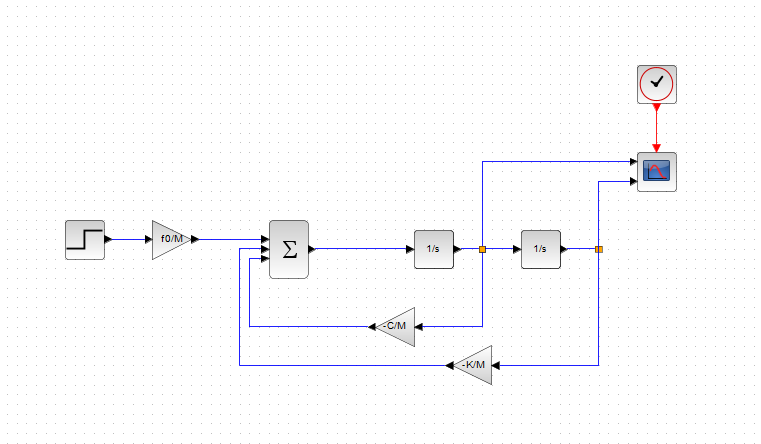
\includegraphics[width=10cm]{../graph/bane-model.png}
  \caption{作成したシミュレーションモデル}
  \label{fig:bane-model.png}
\end{figure}

このとき,左側の積分器の出力が$v(t)$であり,右側の積分器の出力が$x(t)$である.

\subsection{シミュレーションパラメータ値の計算}
使用した各定数は参考文献[1]の指示に従い決定した.
実際に使用した値はそれぞれ次のとおりである.
\begin{itemize}
  \item $m = 出席番号 \times 100$ = 420[kg]
  \item $k = \frac{|150 + (出席番号 - 25)^2 \times 50|}{10} = 1460$[kg/s$^2$]
  \item $c = 650 - (出席番号 - 25)^2 = 361$[kg/s]
  \item $f_o = 300$[kg $\cdot$ cm / s$^2$]
\end{itemize}

\subsection{シミュレーション結果}
各定数を設定したモデルに対し,シミュレーション時間0[s]においてステップ入力1を与え,出力を得た.
変位$x(t)$[cm]及び速度$v(t)$[cm/s]の時間に対するグラフを図\ref{fig:bane-graph.png}に示す.

\begin{figure}[H]
  \centering
  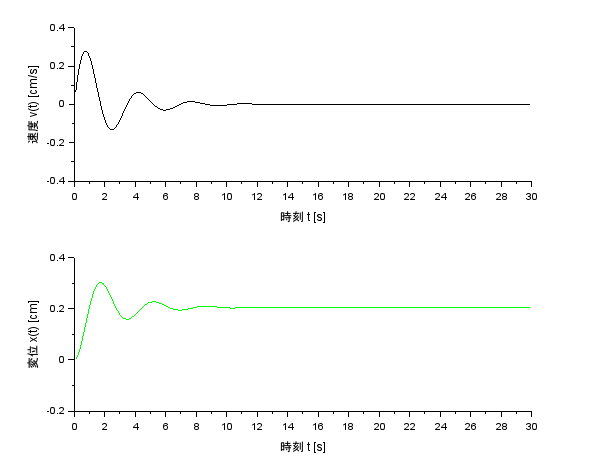
\includegraphics[width=10cm]{../graph/bane-graph.png}
  \caption{系の時間応答シミュレーション結果}
  \label{fig:bane-graph.png}
\end{figure}

\subsection{シミュレーション結果の解析}
まず,質量は正のステップ入力に対し,$x(t)$が正の方向に変位し,また,加速により$v(t)$が正となることは間違いない.
少なくともこの観点には,図2の出力は沿った結果となっている.

次に,定常応答について評価する.
定常応答は,$t \rightarrow \infty$となったときの$x(t)$及び$v(t)$である.
質量は最終的に静止するはずであるから,$v(t)$の定常応答は0となるはずである.
一方,$x(t)$の定常応答は,バネによる弾性力とダンパによる抵抗力のバランスによって決定される.
$x(t)$の定常応答$x_\infty$は,$x_\infty = \frac{f_o}{k}$とすると,
$v(t)$が0となればダンパの抵抗力は発生しなくなることを考えれば,$x_\infty = \frac{300}{1460} = 0.205$[cm]となる.
これら2つの定常応答に対して,図2の出力は沿った結果となっている.

最終的にシミュレーションモデルの結果が正しいか判断するには,これに加え収束までの時間と,周波数について検討する必要があると考えられる.
しかし,今回は時間が足りなかったため,これらの検討は行わなかった.
したがってダンパ成分に対する評価が不十分である.

\section{天井クレーンの制御シミュレーション}
この章では,天井クレーンのPID制御による安定化シミュレーションについて述べる.

数値シミュレーションによる系の制御の実践として,複数の要素が含まれ解析が難しい天井クレーンの安定化を考える.

図 に天井クレーンの構造を示す.
高さ方向$y$,横方向$x$,奥行方向$z$の3軸を考えたとき,一般的な天井クレーンは吊り荷の
移動機構としてそれぞれ巻き上げ機構,トロリ,クレーンガーターを備える.

今回のシミュレーションモデルでは,簡略化のため,クレーンガーター,巻き上げ機構は固定とし,トロリの移動のみを考慮する.
吊り下げる荷重,ロープ長は任意の長さで固定されているものし,
座標系はトロリの移動方向$x$軸,鉛直下向きを$y$軸とする.

このとき,トロリの質量$M$[kg],吊り荷の質量$m$[kg],ロープの長さ$l$[m],
ロープ根本の粘性係数は$\mu$[kg$\cdot m^2$/s]であるとすると,シミュレーションに用いる天井クレーンは
図 のようにモデル化できる.

また,ロープは無視できる質量であるとし,
トロリの変位$x(t)$は右方向を正,吊り荷の揺れ角$\theta(t)$は反時計回りを正とする.
トロリと吊り荷はそれぞれ相互に影響しあい,吊り荷の揺れ角$\theta(t)$はトロリの変位$x(t)$に依存し発生・抑制されるものと考える.

トロリの運動方程式は
\begin{equation}
  \ddot x(t) + \alpha_1 \ddot x(t)+ \alpha_2 \dot x(t) = \beta v(t) \nonumber
\end{equation}
として,内部パラメータとして$\alpha_1$, $\alpha_2$, $\beta$を用いる.

\subsection{天井クレーンの吊り荷部分の運動方程式の導出}
天井クレーンの吊り荷の制振が目的であるから,この部分の運動方程式を導出する.
吊り荷の一般化座標$q(t) = \theta(t)$として,ラグランジュ法を用いて運動方程式を導出する.

運動エネルギ,位置エネルギ,散逸エネルギ,外力によるエネルギの総和を考える.
それぞれ$T$,$U$,$F$,$\tau_i$とし,
ラグラジアン$L = T - U$から,ラグランジュの運動方程式を次のように定義する.
\begin{equation}
  \frac{d}{dt} \frac{\partial T}{\partial \dot{q}} - \frac{\partial T}{\partial q} + \frac{\partial F}{\partial \dot q} + \frac{\partial U}{\partial \dot q} = \tau \nonumber
\end{equation}

外力$\tau$=0として,吊り荷のラグランジュの運動方程式は式(\ref{eq:lagrange})と表せる.
\begin{equation}
  \frac{d}{dt} \frac{\partial T}{\partial \dot{q}} - \frac{\partial T}{\partial q} + \frac{\partial F}{\partial \dot q} + \frac{\partial U}{\partial \dot q} = 0 \label{eq:lagrange}
\end{equation}

各エネルギを導出するため,吊り荷の中心座標を導出する.
ロープが曲がることはないと仮定すると,吊り荷の中心座標$(G_x, G_y)$は,トロリの中心座標$x$と吊り荷の角度$\theta$,ロープ長$l$によって決定される.
このとき,$(G_x, G_y)$は次のとおりである.

\begin{equation}
  \begin{cases}
    G_x = l sin(\theta(t)) + x \nonumber \\
    G_y = l cos(\theta(t))
  \end{cases}
\end{equation}

また,この微分は次のとおりである.
\begin{equation}
  \begin{cases}
    \dot{G_x} = l \dot{\theta(t)} cos(\theta(t)) + \dot x \nonumber \\
    \dot{G_y} = -l \dot{\theta(t)} sin(\theta(t))
  \end{cases}
\end{equation}

中心座標を考慮して吊り荷の運動エネルギ$T$を導出する.
\begin{eqnarray}
  T &=& \frac{1}{2} m (\dot{G_x}^2 + \dot{G_y}^2) + \frac{1}{2}M\dot{x}^2\nonumber \\
  &=& \frac{1}{2} m [ \{l \dot{\theta(t)} cos(\theta(t)) + \dot x\}^2 + \{ -l \dot{\theta(t)} sin(\theta(t))\}^2 ] + \frac{1}{2}M\dot{x}^2 \nonumber \\
  &=& \frac{1}{2} m [\{ \dot x^2 + 2 l \dot{x} \dot{\theta(t)} cos(\theta(t)) + l^2 \dot{\theta(t)}^2 cos^2(\theta(t)) \} + l^2 \dot{\theta(t)}^2 sin^2(\theta(t))] + \frac{1}{2}M\dot{x}^2 \nonumber \\
  &=& \frac{1}{2} m [\dot x^2 + 2 l \dot{x} \dot{\theta(t)} cos(\theta(t)) + l^2 \dot{\theta(t)}^2 \{ cos^2(\theta(t)) + sin^2(\theta(t)) \}] + \frac{1}{2}M\dot{x}^2 \nonumber \\
  &=& \frac{1}{2} m [\dot x^2 + 2 l \dot{x} \dot{\theta(t)} cos(\theta(t)) + l^2 \dot{\theta(t)}^2] + \frac{1}{2}M\dot{x}^2 \nonumber \\
  &=& \frac{1}{2} m \dot x^2 + m l \dot{x} \dot{\theta(t)} cos(\theta(t)) + \frac{1}{2} m l^2 \dot{\theta(t)}^2 + \frac{1}{2}M\dot{x}^2 \nonumber \\
  &=& \frac{1}{2} (M + m)\dot x^2 + m l \dot{x} \dot{\theta(t)} cos(\theta(t)) + \frac{1}{2} m l^2 \dot{\theta(t)}^2 \label{eq:energy}
\end{eqnarray}

同様に,位置エネルギ$U$,散逸エネルギ$F$は次のとおりである.
\begin{eqnarray}
  U &=& mg(l - G_y) \nonumber \\
  &=& mg(l - l cos(\theta(t))) \nonumber \\
  &=& mgl(1 - cos(\theta(t)) \label{eq:potential}\\
\end{eqnarray}

\begin{eqnarray}
  F &=& \frac{1}{2} \mu  \dot{\theta(t)}^2 \label{eq:friction}
\end{eqnarray}

式(\ref{eq:energy}),(\ref{eq:potential}),(\ref{eq:friction})をラグランジュの運動方程式(\ref{eq:lagrange})に代入し,エネルギ式を導く.

ここで各項は,
\begin{eqnarray}
  \frac{d}{dt} \frac{\partial T}{\partial \dot{q}} &=& m l^2 \theta(t) + m l \dot(x) cos(\theta(t)) \nonumber \\
  \frac{\partial T}{\partial \dot{q}} &=&  -m l \dot x \dot{\theta(t)}^2 sin(\theta(t))\nonumber \\
\end{eqnarray}

\begin{eqnarray}
  \frac{d}{dt} \frac{\partial F}{\partial \dot{q}} &=&  \mu \dot{\theta(t)} \nonumber \\
  \frac{\partial U}{\partial \dot{q}} &=&  mgl sin(\theta(t)) \nonumber \\
\end{eqnarray}

であるから,求める運動方程式は
\begin{eqnarray}
  \frac{d}{dt} \frac{\partial T}{\partial \dot{q}} - \frac{\partial T}{\partial q} + \frac{\partial F}{\partial \dot q} + \frac{\partial U}{\partial \dot q} = 0 \nonumber \\
  m l^2 \theta(t) + m l \dot x cos(\theta(t)) + m l \dot x \dot{\theta(t)}^2 sin(\theta(t)) + \mu \dot{\theta(t)} + mgl sin(\theta(t)) = 0 \nonumber \\
\end{eqnarray}

\subsection{シミュレーションパラメータの計算}
構成したシミュレーションモデルの構造を図 に示す.

モデル上の各シミュレーションパラメータは参考文献[1]の指示に従い決定した.
実際に使用したパラメータはそれぞれ次のとおりである.
\begin{itemize}
  \item $m = 0.5 + (\frac{出席番号 - 25}{10})^2 = 3.39$
  \item $l = 0.16 + (出席番号 \times 0.04) = 1.84$
  \item $\alpha_1 = 37.2$
  \item $\alpha_2 = 1980$
  \item $\beta = 180$
  \item $\mu = 1.22 \times  10^{-3}$
\end{itemize}

\subsection{設計仕様を満たすPID制御器の設計とシミュレーション結果}
設計したPID制御器について述べる.
今回のシミュレーションでは,目標位置に向けてトロリの制動速度を制御するPID制御器,吊り荷の揺れ角によってトロリの速度を制御するPID制御器の2つを考える.

前者は,目標位置が近づくにつれてトロリの制動速度を減速させることで,目標位置に到達するまでの時間を効率的に短縮する等の役割を担う.
後者は,吊り荷の揺れ角が大きくなるにつれてトロリの速度を減速させることで,吊り荷の揺れ角を小さくする等の役割を担う.

両PID制御器の設計仕様は次のとおりである.
参考資料[1]の内容に加え,項目3に整定条件を追加している.

\begin{enumerate}
  \item トロリは目標位置の印加後5[sec]以内で整定し,オーバーシュートを5\%以内とする.
  \item 吊り荷の揺れ角は$\pm$7[deg]以内とする.
  \item 整定条件は$\pm$2[\%]以内とする.
\end{enumerate}

\paragraph{シミュレーションによるパラメータ同定}

目標位置に向けてトロリの制動速度を制御するPID制御器のPIDパラメータ$P_1$, $I_1$, $D_1$,
吊り荷の揺れ角によってトロリの速度を制御するPID制御器のPIDパラメータ$P_2$, $I_2$, $D_2$として,シミュレーション上でパラメータ同定を行った.

同定した最終的なPIDパラメータ及びモデルの時間変化を図\ref{fig:crane:fin-up}に示す.

\begin{figure}[H]
  \begin{minipage}{4.5cm}
    \centering
    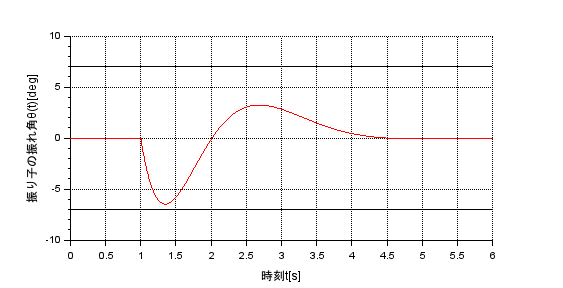
\includegraphics[keepaspectratio, scale=0.35]{../graph/crane/ang-fin-up.png}
    \subcaption{吊り荷の揺れ角の時間変化}
  \end{minipage}
  \hfill
  \begin{minipage}{4.5cm}
    \centering
    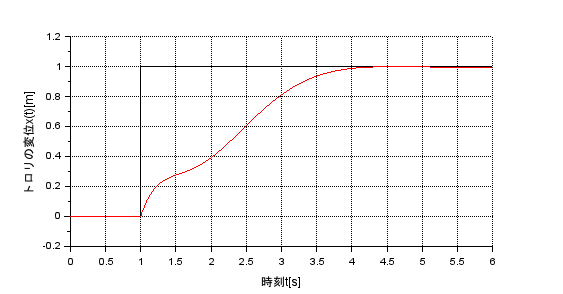
\includegraphics[keepaspectratio, scale=0.35]{../graph/crane/po-fin-up.png}
    \subcaption{トロリの変位の時間変化}
  \end{minipage}
  \hfill
  \begin{minipage}{3cm}
      \begin{center}
        \begin{tabular}{c|c}
          \hline
          $P_1$ & 300\\ \hline
          $I_1$ & 0\\ \hline
          $D_1$ & 200\\ \hline
          $P_2$ & 1150\\ \hline
          $I_2$ & 1500\\ \hline
          $D_2$ & 0\\
          \hline
        \end{tabular}
      \end{center}
  \end{minipage}
  \hfill
  \caption{同定したパラメータによって制御した場合のクレーンモデルの時間変化}
  \label{fig:crane:fin-up}
\end{figure}

\paragraph{パラメータ同定における試行過程と方法}
上記パラメータを導くにあたって行った試行の方法について述べる.
まず,パラメータ同定までの過程を示す.
\begin{enumerate}
  \item 全パラメータを0としてシミュレーションを実施
  \item 各PIDパラメータに任意の値を入力し,各パラメータの挙動を観察
  \item 6つのパラメータのうち,使い物にならないパラメータを決定
  \item バランスの良いパラメータを固定し,残りのパラメータを調整
  \item 2つのPID制御器のパラメータを相互に微調整
\end{enumerate}

\paragraph{全パラメータを0としてシミュレーションを実施\\}
図\ref{fig:crane:0}に全パラメータを0とした場合のシミュレーション結果を示す.

\begin{figure}[H]
  \begin{minipage}{4.5cm}
    \centering
    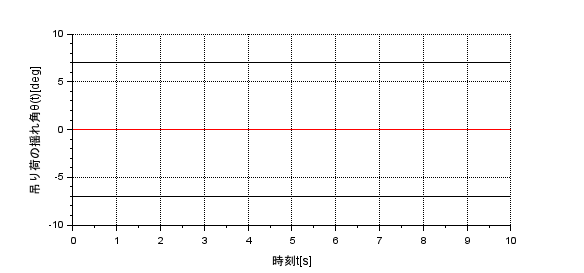
\includegraphics[keepaspectratio, scale=0.35]{../graph/crane/ang-0.png}
    \subcaption{吊り荷の揺れ角の時間変化}
  \end{minipage}
  \hfill
  \begin{minipage}{4.5cm}
    \centering
    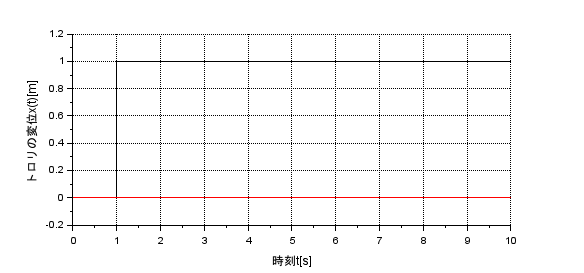
\includegraphics[keepaspectratio, scale=0.35]{../graph/crane/po-0.png}
    \subcaption{トロリの変位の時間変化}
  \end{minipage}
  \hfill
  \begin{minipage}{3cm}
    \begin{center}
      \begin{tabular}{c|c}
        \hline
        $P_1$ & 0\\ \hline
        $I_1$ & 0\\ \hline
        $D_1$ & 0\\ \hline
        $P_2$ & 0\\ \hline
        $I_2$ & 0\\ \hline
        $D_2$ & 0\\
        \hline
      \end{tabular}
    \end{center}
  \end{minipage}
  \hfill
  \caption{PID制御器のパラメータを全て0にした場合}
  \label{fig:crane:0}
\end{figure}

図\ref{fig:crane:0}から,全パラメータが0の場合は,系は反応を返さないことがわかる,
入力$e(t)$,出力$u(t)$とするとPID制御は以下の式で表されるため,この応答は当然の挙動である.
\begin{equation}
  u(t) = P_1 e(t) + I_1 \int_0^t e(\tau) d\tau + D_1 \frac{de(t)}{dt} \nonumber
\end{equation}

\paragraph{各PIDパラメータに任意の値を入力し,各パラメータの挙動を観察\\}
各パラメータが吊り荷及びトロリの運動の時間変化に与える影響を観察するため,
各パラメータに任意の値を入力しシミュレーションを実施した.

はじめに,吊り荷の揺れ角によってトロリの速度を制御するPID制御器のパラメータはすべて0とし,
トロリの変位によってトロリの速度を制御するPID制御器のパラメータを変化させた.

$P_1$に5を入力し,得た応答を図\ref{fig:crane:1}に示す.
\begin{figure}[H]
  \begin{minipage}{4.5cm}
    \centering
    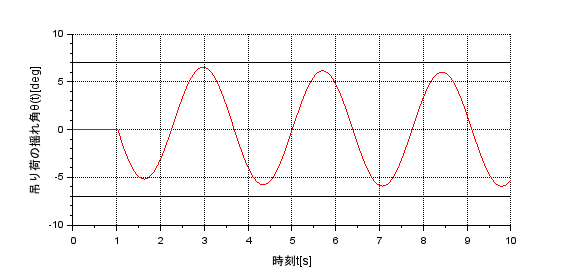
\includegraphics[keepaspectratio, scale=0.35]{../graph/crane/ang-P1-5-I1-0-D1-0-P2-0-I2-0-D2-0.png}
    \subcaption{吊り荷の揺れ角の時間変化}
  \end{minipage}
  \hfill
  \begin{minipage}{4.5cm}
    \centering
    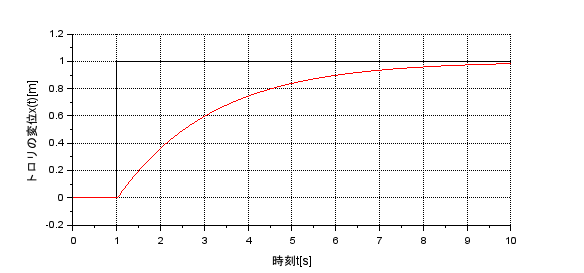
\includegraphics[keepaspectratio, scale=0.35]{../graph/crane/po-P1-5-I1-0-D1-0-P2-0-I2-0-D2-0.png}
    \subcaption{トロリの変位の時間変化}
  \end{minipage}
  \hfill
  \begin{minipage}{3cm}
    \begin{center}
      \begin{tabular}{c|c}
        \hline
        $P_1$ & 5\\ \hline
        $I_1$ & 0\\ \hline
        $D_1$ & 0\\ \hline
        $P_2$ & 0\\ \hline
        $I_2$ & 0\\ \hline
        $D_2$ & 0\\
        \hline
      \end{tabular}
    \end{center}
  \end{minipage}
  \hfill
  \caption{$P_1$パラメータを5にした場合}
  \label{fig:crane:1}
\end{figure}

図\ref{fig:crane:1}から,比例項である$P_1$パラメータを入力すると,トロリは目標値に向かって変位を増大させることがわかる.
設計仕様1を満たすため,トロリの目標値到達高速化を狙い,$P_1$パラメータを増加させ実験する.

$P_1$に100を入力し得た応答を図\ref{fig:crane:2}に,300を入力し得た応答を図\ref{fig:crane:2}に示す.

\begin{figure}[H]
  \begin{minipage}{4.5cm}
    \centering
    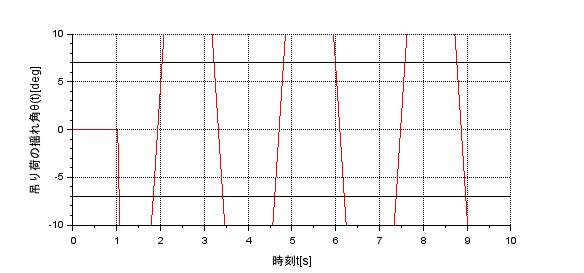
\includegraphics[keepaspectratio, scale=0.35]{../graph/crane/ang-P1-100-I1-0-D1-0-P2-0-I2-0-D2-0.png}
    \subcaption{吊り荷の揺れ角の時間変化}
  \end{minipage}
  \hfill
  \begin{minipage}{4.5cm}
    \centering
    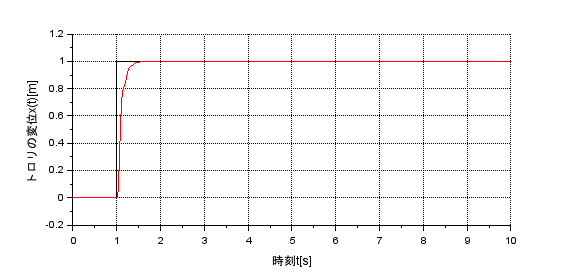
\includegraphics[keepaspectratio, scale=0.35]{../graph/crane/po-P1-100-I1-0-D1-0-P2-0-I2-0-D2-0.png}
    \subcaption{トロリの変位の時間変化}
  \end{minipage}
  \hfill
  \begin{minipage}{3cm}
    \begin{center}
      \begin{tabular}{c|c}
        \hline
        $P_1$ & 100\\ \hline
        $I_1$ & 0\\ \hline
        $D_1$ & 0\\ \hline
        $P_2$ & 0\\ \hline
        $I_2$ & 0\\ \hline
        $D_2$ & 0\\
        \hline
      \end{tabular}
    \end{center}
  \end{minipage}
  \hfill
  \caption{$P_1$パラメータを100にした場合}
  \label{fig:crane:2}
\end{figure}

\begin{figure}[H]
  \begin{minipage}{4.5cm}
    \centering
    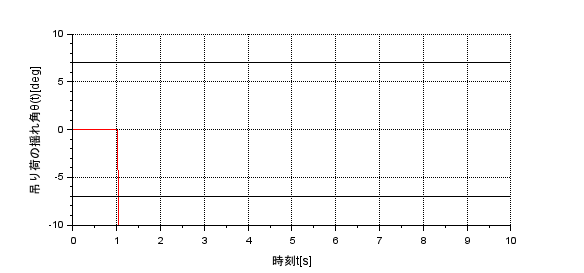
\includegraphics[keepaspectratio, scale=0.35]{../graph/crane/ang-P1-300-I1-0-D1-0-P2-0-I2-0-D2-0.png}
    \subcaption{吊り荷の揺れ角の時間変化}
  \end{minipage}
  \hfill
  \begin{minipage}{4.5cm}
    \centering
    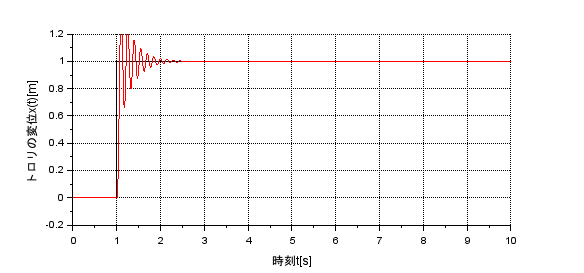
\includegraphics[keepaspectratio, scale=0.35]{../graph/crane/po-P1-300-I1-0-D1-0-P2-0-I2-0-D2-0.png}
    \subcaption{トロリの変位の時間変化}
  \end{minipage}
  \hfill
  \begin{minipage}{3cm}
    \begin{center}
      \begin{tabular}{c|c}
        \hline
        $P_1$ & 300\\ \hline
        $I_1$ & 0\\ \hline
        $D_1$ & 0\\ \hline
        $P_2$ & 0\\ \hline
        $I_2$ & 0\\ \hline
        $D_2$ & 0\\
        \hline
      \end{tabular}
    \end{center}
  \end{minipage}
  \hfill
  \caption{$P_1$パラメータを300にした場合}
  \label{fig:crane:3}
\end{figure}

図\ref{fig:crane:2}と図\ref{fig:crane:3}から,$P_1$パラメータの増加はトロリの目標値到達高速化を可能とすることがわかる.
弊害として,吊り荷の揺れ角も増大するため,設計仕様2を満たすことができないことも確認できる.
$P_1 = 300$では,収束前の1[s]から2[s]において発振が発生していることが確認できる.

この発振は設計仕様1,3を同時に満たすために不都合であるため,$I_1$,$D_1$パラメータによって発振を抑制可能か確認した.

\begin{figure}[H]
  \begin{minipage}{4.5cm}
    \centering
    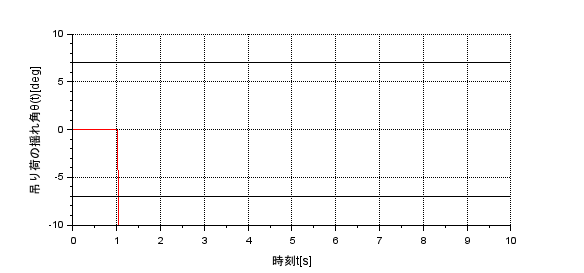
\includegraphics[keepaspectratio, scale=0.35]{../graph/crane/ang-P1-300-I1-0-D1-0-P2-0-I2-0-D2-0.png}
    \subcaption{吊り荷の揺れ角の時間変化}
  \end{minipage}
  \hfill
  \begin{minipage}{4.5cm}
    \centering
    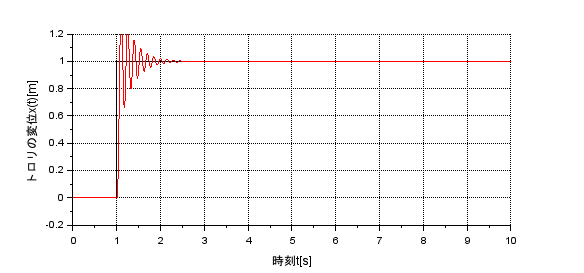
\includegraphics[keepaspectratio, scale=0.35]{../graph/crane/po-P1-300-I1-0-D1-0-P2-0-I2-0-D2-0.png}
    \subcaption{トロリの変位の時間変化}
  \end{minipage}
  \hfill
  \begin{minipage}{3cm}
    \begin{center}
      \begin{tabular}{c|c}
        \hline
        $P_1$ & 300\\ \hline
        $I_1$ & 0\\ \hline
        $D_1$ & 0\\ \hline
        $P_2$ & 0\\ \hline
        $I_2$ & 0\\ \hline
        $D_2$ & 0\\
        \hline
      \end{tabular}
    \end{center}
  \end{minipage}
  \hfill
  \caption{$I_1$パラメータを100を追加した場合}
  \label{fig:crane:4}
\end{figure}

\begin{figure}[H]
  \begin{minipage}{4.5cm}
    \centering
    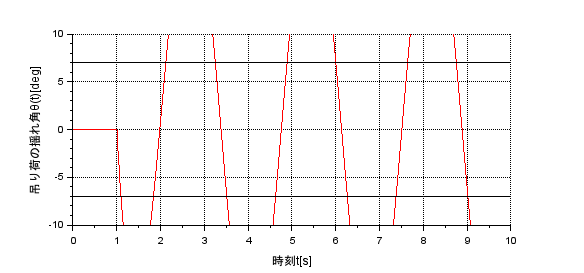
\includegraphics[keepaspectratio, scale=0.35]{../graph/crane/ang-P1-300-I1-0-D1-100-P2-0-I2-0-D2-0.png}
    \subcaption{吊り荷の揺れ角の時間変化}
  \end{minipage}
  \hfill
  \begin{minipage}{4.5cm}
    \centering
    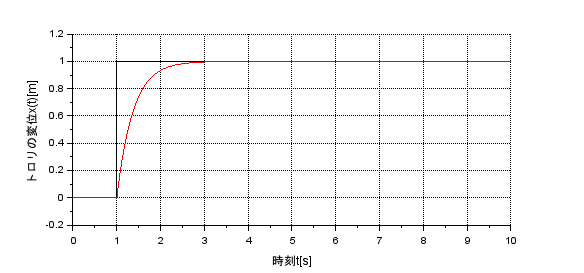
\includegraphics[keepaspectratio, scale=0.35]{../graph/crane/po-P1-300-I1-0-D1-100-P2-0-I2-0-D2-0.png}
    \subcaption{トロリの変位の時間変化}
  \end{minipage}
  \hfill
  \begin{minipage}{3cm}
    \begin{center}
      \begin{tabular}{c|c}
        \hline
        $P_1$ & 300\\ \hline
        $I_1$ & 0\\ \hline
        $D_1$ & 100\\ \hline
        $P_2$ & 0\\ \hline
        $I_2$ & 0\\ \hline
        $D_2$ & 0\\
        \hline
      \end{tabular}
    \end{center}
  \end{minipage}
  \hfill
  \caption{$D_1$パラメータに100を追加した場合}
  \label{fig:crane:5}
\end{figure}

\begin{figure}[H]
  \begin{minipage}{4.5cm}
    \centering
    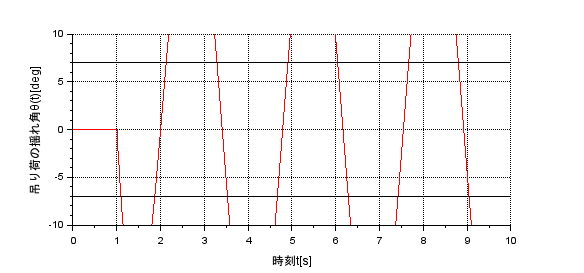
\includegraphics[keepaspectratio, scale=0.35]{../graph/crane/ang-P1-300-I1-100-D1-0-P2-0-I2-0-D2-0.png}
    \subcaption{吊り荷の揺れ角の時間変化}
  \end{minipage}
  \hfill
  \begin{minipage}{4.5cm}
    \centering
    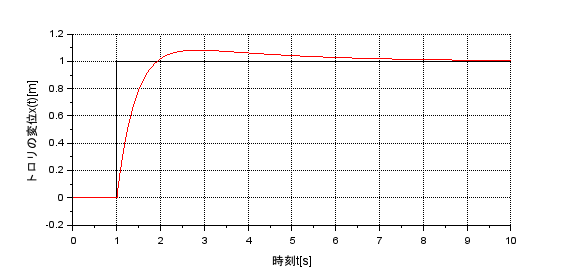
\includegraphics[keepaspectratio, scale=0.35]{../graph/crane/po-P1-300-I1-100-D1-0-P2-0-I2-0-D2-0.png}
    \subcaption{トロリの変位の時間変化}
  \end{minipage}
  \hfill
  \begin{minipage}{3cm}
    \begin{center}
      \begin{tabular}{c|c}
        \hline
        $P_1$ & 300\\ \hline
        $I_1$ & 100\\ \hline
        $D_1$ & 100\\ \hline
        $P_2$ & 0\\ \hline
        $I_2$ & 0\\ \hline
        $D_2$ & 0\\
        \hline
      \end{tabular}
    \end{center}
  \end{minipage}
  \hfill
  \caption{$I_1$,$D_1$パラメータに100を追加した場合}
  \label{fig:crane:6}
\end{figure}

図\ref{fig:crane:4}より,$I_1$パラメータは発振の抑制に効果がないこと.
図\ref{fig:crane:5}より,$D_1$パラメータが発振の抑制に効果的であることがわかった.

図\ref{fig:crane:6}のとおり$I_1$パラメータを追加したが,トロリの時間変化の収束位置が目標値を超えてしまうため,
今回のモデルの制御に不適であると判断し,今後$P_1 = 300$,$D_1 = 100$を基本とし調整していくこととした.

\paragraph{吊り荷の揺れ角によってトロリの速度を制御するPID制御器の調整\\}
トロリの変位によってトロリの速度を制御するPID制御器のパラメータを先述したとおり$P_1 = 300$,$I_1 = 0$,$D_1 = 100$に固定し,
吊り荷の揺れ角によってトロリの速度を制御するPID制御器の調整を行う.

はじめに,設計仕様2を満たすため,揺れ角の抑制を狙い,$P_2$パラメータを増加させ実験する.
$P_2 = 100$とした出力を図\ref{fig:crane:7}に示す.

\begin{figure}[H]
  \begin{minipage}{4.5cm}
    \centering
    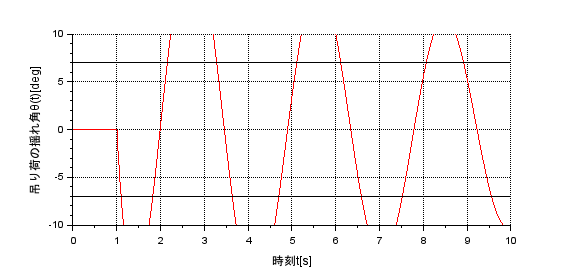
\includegraphics[keepaspectratio, scale=0.35]{../graph/crane/ang-P1-300-I1-0-D1-100-P2-100-I2-0-D2-0.png}
    \subcaption{吊り荷の揺れ角の時間変化}
  \end{minipage}
  \hfill
  \begin{minipage}{4.5cm}
    \centering
    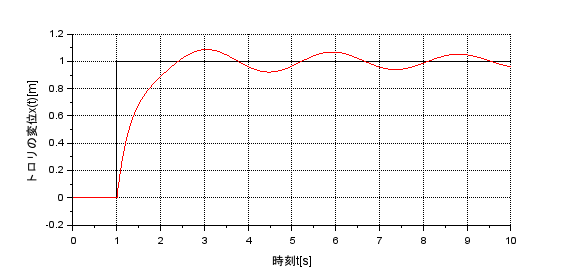
\includegraphics[keepaspectratio, scale=0.35]{../graph/crane/po-P1-300-I1-0-D1-100-P2-100-I2-0-D2-0.png}
    \subcaption{トロリの変位の時間変化}
  \end{minipage}
  \hfill
  \begin{minipage}{3cm}
    \begin{center}
      \begin{tabular}{c|c}
        \hline
        $P_1$ & 300\\ \hline
        $I_1$ & 0\\ \hline
        $D_1$ & 100\\ \hline
        $P_2$ & 100\\ \hline
        $I_2$ & 0\\ \hline
        $D_2$ & 0\\
        \hline
      \end{tabular}
    \end{center}
  \end{minipage}
  \hfill
  \caption{$P_2$,パラメータに100を追加した場合}
  \label{fig:crane:7}
\end{figure}

図\ref{fig:crane:7}より,図\ref{fig:crane:5}と比較して揺れ角が抑制できている様子が確認できる.
しかしながら,吊り荷の影響でトロリの運動が被直線的となる弊害が確認された.
トロリの変位によってトロリの速度を制御するPID制御器のパラメータ調整では,発振の抑制に$D$パラメータが効果的であったため,
揺れ角抑制にも利用できると予想し,$D_2$パラメータに100を入力した.
出力を図\ref{fig:crane:8}に示す.

\begin{figure}[H]
  \begin{minipage}{4.5cm}
    \centering
    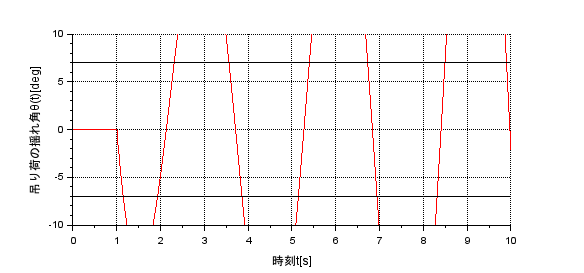
\includegraphics[keepaspectratio, scale=0.35]{../graph/crane/po-P1-300-I1-0-D1-100-P2-100-I2-0-D2-100.png}
    \subcaption{吊り荷の揺れ角の時間変化}
  \end{minipage}
  \hfill
  \begin{minipage}{4.5cm}
    \centering
    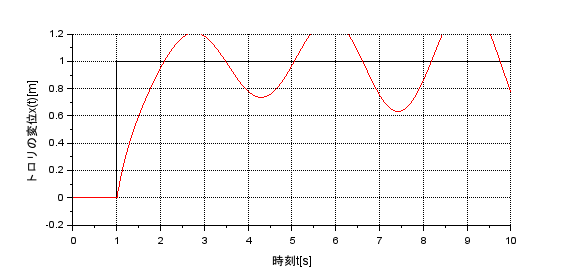
\includegraphics[keepaspectratio, scale=0.35]{../graph/crane/ang-P1-300-I1-0-D1-100-P2-100-I2-0-D2-100.png}
    \subcaption{トロリの変位の時間変化}
  \end{minipage}
  \hfill
  \begin{minipage}{3cm}
    \begin{center}
      \begin{tabular}{c|c}
        \hline
        $P_1$ & 300\\ \hline
        $I_1$ & 0\\ \hline
        $D_1$ & 100\\ \hline
        $P_2$ & 100\\ \hline
        $I_2$ & 0\\ \hline
        $D_2$ & 100\\
        \hline
      \end{tabular}
    \end{center}
  \end{minipage}
  \hfill
  \caption{$D_2$,パラメータに100を追加した場合}
  \label{fig:crane:8}
\end{figure}

図\ref{fig:crane:8}より,予想に反し$D_2$パラメータはかえって揺れ角を増大させてしまっていることがわかる.
同様の理由で$I_2$パラメータに100を入力し試行した.

------------

\begin{figure}[H]
  \begin{minipage}{4.5cm}
    \centering
    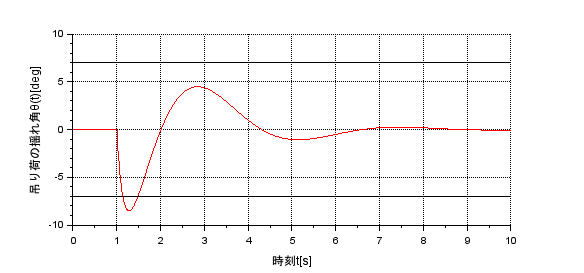
\includegraphics[keepaspectratio, scale=0.35]{../graph/crane/ang-P1-300-I1-0-D1-100-P2-1000-I2-1000-D2-0.png}
    \subcaption{吊り荷の揺れ角の時間変化}
  \end{minipage}
  \hfill
  \begin{minipage}{4.5cm}
    \centering
    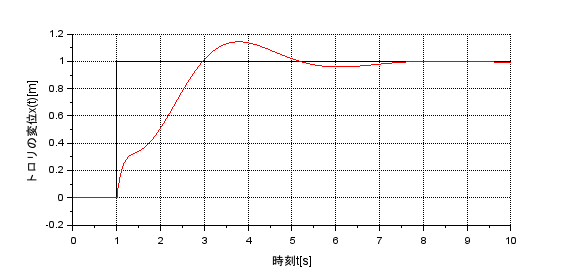
\includegraphics[keepaspectratio, scale=0.35]{../graph/crane/po-P1-300-I1-0-D1-100-P2-1000-I2-1000-D2-0.png}
    \subcaption{トロリの変位の時間変化}
  \end{minipage}
  \hfill
  \begin{minipage}{3cm}
    \begin{center}
      \begin{tabular}{c|c}
        \hline
        $P_1$ & 300\\ \hline
        $I_1$ & 0\\ \hline
        $D_1$ & 100\\ \hline
        $P_2$ & 1000\\ \hline
        $I_2$ & 1000\\ \hline
        $D_2$ & 0\\
        \hline
      \end{tabular}
    \end{center}
  \end{minipage}
  \hfill
  \caption{$D_2$,パラメータに1000を追加した場合}
  \label{fig:crane:10}
\end{figure}

図\ref{fig:crane:10}より,収束時間の特性が向上していることが確認できる.
トロリ収束前に発生している波を軽減するため,低速な発振とみなし$I_2$パラメータを用いることを考えた.
直線的な運動となるまで$D_1$を1000,1500と増加させた出力を図\ref{fig:crane:11},図\ref{fig:crane:12}に示す.

\begin{figure}[H]
  \begin{minipage}{4.5cm}
    \centering
    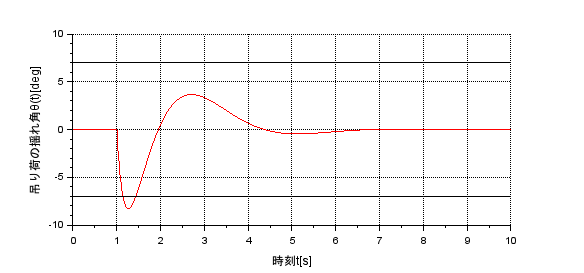
\includegraphics[keepaspectratio, scale=0.35]{../graph/crane/ang-P1-300-I1-0-D1-100-P2-1000-I2-1500-D2-0.png}
    \subcaption{吊り荷の揺れ角の時間変化}
  \end{minipage}
  \hfill
  \begin{minipage}{4.5cm}
    \centering
    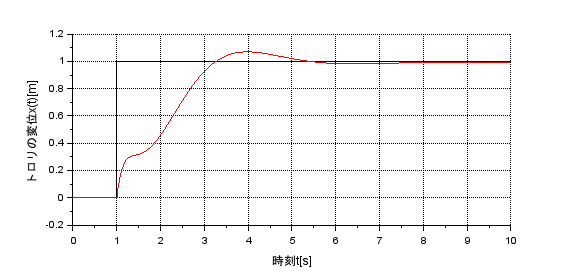
\includegraphics[keepaspectratio, scale=0.35]{../graph/crane/po-P1-300-I1-0-D1-100-P2-1000-I2-1500-D2-0.png}
    \subcaption{トロリの変位の時間変化}
  \end{minipage}
  \hfill
  \begin{minipage}{3cm}
    \begin{center}
      \begin{tabular}{c|c}
        \hline
        $P_1$ & 300\\ \hline
        $I_1$ & 0\\ \hline
        $D_1$ & 100\\ \hline
        $P_2$ & 1000\\ \hline
        $I_2$ & 1500\\ \hline
        $D_2$ & 0\\
        \hline
      \end{tabular}
    \end{center}
  \end{minipage}
  \hfill
  \caption{$D_2$パラメータに1500を変更した場合}
  \label{fig:crane:11}
\end{figure}

\paragraph{2つのPID制御器のパラメータを相互に微調整\\}
前項目の$I_2$にの変更だけではトロリ収束前に発生している波を十分に減少させることはできなかった.

そこで発振を軽減可能な$D_1$パラメータを微調整し,より直線的な運動となる点を検討したところ,$D_1 = 200$にて十分な効果が得られた.
出力を図\ref{fig:crane:11}に示す.

\begin{figure}[H]
  \begin{minipage}{4.5cm}
    \centering
    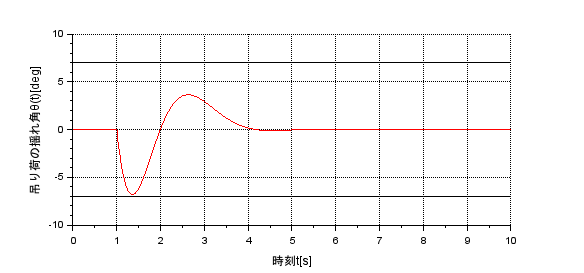
\includegraphics[keepaspectratio, scale=0.35]{../graph/crane/ang-P1-300-I1-0-D1-200-P2-1000-I2-1500-D2-0.png}
    \subcaption{吊り荷の揺れ角の時間変化}
  \end{minipage}
  \hfill
  \begin{minipage}{4.5cm}
    \centering
    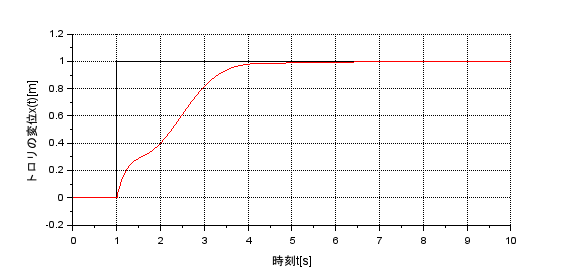
\includegraphics[keepaspectratio, scale=0.35]{../graph/crane/po-P1-300-I1-0-D1-200-P2-1000-I2-1500-D2-0.png}
    \subcaption{トロリの変位の時間変化}
  \end{minipage}
  \hfill
  \begin{minipage}{3cm}
    \begin{center}
      \begin{tabular}{c|c}
        \hline
        $P_1$ & 300\\ \hline
        $I_1$ & 0\\ \hline
        $D_1$ & 200\\ \hline
        $P_2$ & 1000\\ \hline
        $I_2$ & 1500\\ \hline
        $D_2$ & 0\\
        \hline
      \end{tabular}
    \end{center}
  \end{minipage}
  \hfill
  \caption{$D_1$パラメータを200を変更した場合}
  \label{fig:crane:11}
\end{figure}

図\ref{fig:crane:11}では,立ち上がり時4[s]から6[s]まで目標値に漸近しているが改善可能と見られる領域が残されている.
$P_1$パラメータを増加させることで変位の増加を図り,最終パラメータを得た.
改めて図\ref{fig:crane:final}に示す.

\begin{figure}[H]
  \begin{minipage}{4.5cm}
    \centering
    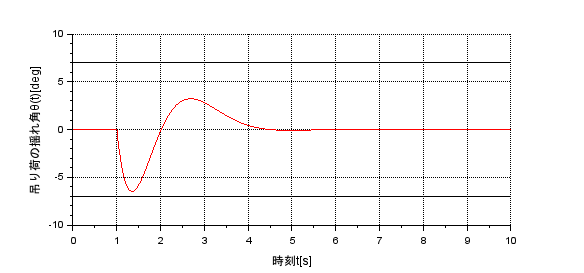
\includegraphics[keepaspectratio, scale=0.35]{../graph/crane/ang-final.png}
    \subcaption{吊り荷の揺れ角の時間変化}
  \end{minipage}
  \hfill
  \begin{minipage}{4.5cm}
    \centering
    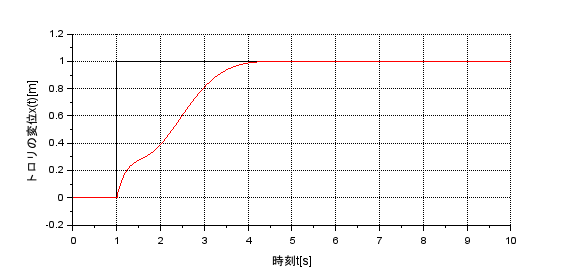
\includegraphics[keepaspectratio, scale=0.35]{../graph/crane/po-final.png}
    \subcaption{トロリの変位の時間変化}
  \end{minipage}
  \hfill
  \begin{minipage}{3cm}
      \begin{center}
        \begin{tabular}{c|c}
          \hline
          $P_1$ & 300\\ \hline
          $I_1$ & 0\\ \hline
          $D_1$ & 200\\ \hline
          $P_2$ & 1150\\ \hline
          $I_2$ & 1500\\ \hline
          $D_2$ & 0\\
          \hline
        \end{tabular}
      \end{center}
  \end{minipage}
  \hfill
  \caption{同定したパラメータによって得られた出力}
  \label{fig:crane:final}
\end{figure}

最終出力(図\ref{fig:crane:final})の収束部を拡大したものを図\ref{fig:crane:max}示す.

\begin{figure}[H]
  \begin{minipage}{4.5cm}
    \centering
    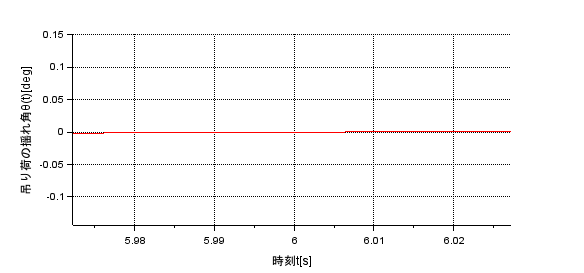
\includegraphics[keepaspectratio, scale=0.35]{../graph/crane/ang-max.png}
    \subcaption{吊り荷の揺れ角の時間変化}
  \end{minipage}
  \hfill
  \begin{minipage}{4.5cm}
    \centering
    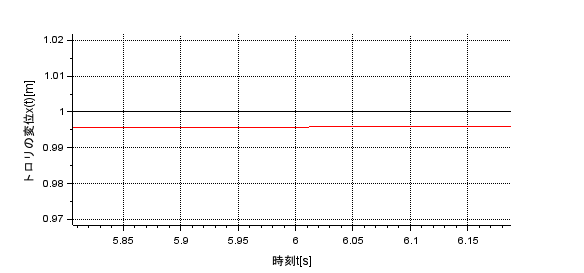
\includegraphics[keepaspectratio, scale=0.35]{../graph/crane/po-max.png}
    \subcaption{トロリの変位の時間変化}
  \end{minipage}
  \hfill
  \begin{minipage}{3cm}
      \begin{center}
        \begin{tabular}{c|c}
          \hline
          $P_1$ & 300\\ \hline
          $I_1$ & 0\\ \hline
          $D_1$ & 200\\ \hline
          $P_2$ & 1150\\ \hline
          $I_2$ & 1500\\ \hline
          $D_2$ & 0\\
          \hline
        \end{tabular}
      \end{center}
  \end{minipage}
  \hfill
  \caption{6.0[s]での収束部周辺を拡大したグラフ}
  \label{fig:crane:max}
\end{figure}

図\ref{fig:crane:max}のとおり,収束時には完全に一致しているわけではないことが確認できる.
一般的に整定条件は2\%または5\%という記述に従い,設定した設計仕様3より,吊り荷の時間変化ほぼ一致,トロリの時間変化0.995[m]より
この誤差を許容する.

この誤差の大きさをどこまで許容するかについては,モデルを用いるユースケースによって別途検討する必要があると考える.

\section{感想}

\begin{thebibliography}{99}
  \bibitem{ataka} 佐藤 拓史、実験テキスト「数値シュミレーション」、(2022年),
\end{thebibliography}

\end{document}